\documentclass[12pt,a4paper]{article}

\usepackage[a4paper,text={16.5cm,25.2cm},centering]{geometry}
\usepackage{lmodern}
\usepackage{amssymb,amsmath}
\usepackage{bm}
\usepackage{graphicx}
\usepackage{microtype}
\usepackage{hyperref}
\setlength{\parindent}{0pt}
\setlength{\parskip}{1.2ex}

\hypersetup
       {   pdfauthor = { Sheehan Olver },
           pdftitle={ foo },
           colorlinks=TRUE,
           linkcolor=black,
           citecolor=blue,
           urlcolor=blue
       }




\usepackage{upquote}
\usepackage{listings}
\usepackage{xcolor}
\lstset{
    basicstyle=\ttfamily\footnotesize,
    upquote=true,
    breaklines=true,
    breakindent=0pt,
    keepspaces=true,
    showspaces=false,
    columns=fullflexible,
    showtabs=false,
    showstringspaces=false,
    escapeinside={(*@}{@*)},
    extendedchars=true,
}
\newcommand{\HLJLt}[1]{#1}
\newcommand{\HLJLw}[1]{#1}
\newcommand{\HLJLe}[1]{#1}
\newcommand{\HLJLeB}[1]{#1}
\newcommand{\HLJLo}[1]{#1}
\newcommand{\HLJLk}[1]{\textcolor[RGB]{148,91,176}{\textbf{#1}}}
\newcommand{\HLJLkc}[1]{\textcolor[RGB]{59,151,46}{\textit{#1}}}
\newcommand{\HLJLkd}[1]{\textcolor[RGB]{214,102,97}{\textit{#1}}}
\newcommand{\HLJLkn}[1]{\textcolor[RGB]{148,91,176}{\textbf{#1}}}
\newcommand{\HLJLkp}[1]{\textcolor[RGB]{148,91,176}{\textbf{#1}}}
\newcommand{\HLJLkr}[1]{\textcolor[RGB]{148,91,176}{\textbf{#1}}}
\newcommand{\HLJLkt}[1]{\textcolor[RGB]{148,91,176}{\textbf{#1}}}
\newcommand{\HLJLn}[1]{#1}
\newcommand{\HLJLna}[1]{#1}
\newcommand{\HLJLnb}[1]{#1}
\newcommand{\HLJLnbp}[1]{#1}
\newcommand{\HLJLnc}[1]{#1}
\newcommand{\HLJLncB}[1]{#1}
\newcommand{\HLJLnd}[1]{\textcolor[RGB]{214,102,97}{#1}}
\newcommand{\HLJLne}[1]{#1}
\newcommand{\HLJLneB}[1]{#1}
\newcommand{\HLJLnf}[1]{\textcolor[RGB]{66,102,213}{#1}}
\newcommand{\HLJLnfm}[1]{\textcolor[RGB]{66,102,213}{#1}}
\newcommand{\HLJLnp}[1]{#1}
\newcommand{\HLJLnl}[1]{#1}
\newcommand{\HLJLnn}[1]{#1}
\newcommand{\HLJLno}[1]{#1}
\newcommand{\HLJLnt}[1]{#1}
\newcommand{\HLJLnv}[1]{#1}
\newcommand{\HLJLnvc}[1]{#1}
\newcommand{\HLJLnvg}[1]{#1}
\newcommand{\HLJLnvi}[1]{#1}
\newcommand{\HLJLnvm}[1]{#1}
\newcommand{\HLJLl}[1]{#1}
\newcommand{\HLJLld}[1]{\textcolor[RGB]{148,91,176}{\textit{#1}}}
\newcommand{\HLJLs}[1]{\textcolor[RGB]{201,61,57}{#1}}
\newcommand{\HLJLsa}[1]{\textcolor[RGB]{201,61,57}{#1}}
\newcommand{\HLJLsb}[1]{\textcolor[RGB]{201,61,57}{#1}}
\newcommand{\HLJLsc}[1]{\textcolor[RGB]{201,61,57}{#1}}
\newcommand{\HLJLsd}[1]{\textcolor[RGB]{201,61,57}{#1}}
\newcommand{\HLJLsdB}[1]{\textcolor[RGB]{201,61,57}{#1}}
\newcommand{\HLJLsdC}[1]{\textcolor[RGB]{201,61,57}{#1}}
\newcommand{\HLJLse}[1]{\textcolor[RGB]{59,151,46}{#1}}
\newcommand{\HLJLsh}[1]{\textcolor[RGB]{201,61,57}{#1}}
\newcommand{\HLJLsi}[1]{#1}
\newcommand{\HLJLso}[1]{\textcolor[RGB]{201,61,57}{#1}}
\newcommand{\HLJLsr}[1]{\textcolor[RGB]{201,61,57}{#1}}
\newcommand{\HLJLss}[1]{\textcolor[RGB]{201,61,57}{#1}}
\newcommand{\HLJLssB}[1]{\textcolor[RGB]{201,61,57}{#1}}
\newcommand{\HLJLnB}[1]{\textcolor[RGB]{59,151,46}{#1}}
\newcommand{\HLJLnbB}[1]{\textcolor[RGB]{59,151,46}{#1}}
\newcommand{\HLJLnfB}[1]{\textcolor[RGB]{59,151,46}{#1}}
\newcommand{\HLJLnh}[1]{\textcolor[RGB]{59,151,46}{#1}}
\newcommand{\HLJLni}[1]{\textcolor[RGB]{59,151,46}{#1}}
\newcommand{\HLJLnil}[1]{\textcolor[RGB]{59,151,46}{#1}}
\newcommand{\HLJLnoB}[1]{\textcolor[RGB]{59,151,46}{#1}}
\newcommand{\HLJLoB}[1]{\textcolor[RGB]{102,102,102}{\textbf{#1}}}
\newcommand{\HLJLow}[1]{\textcolor[RGB]{102,102,102}{\textbf{#1}}}
\newcommand{\HLJLp}[1]{#1}
\newcommand{\HLJLc}[1]{\textcolor[RGB]{153,153,119}{\textit{#1}}}
\newcommand{\HLJLch}[1]{\textcolor[RGB]{153,153,119}{\textit{#1}}}
\newcommand{\HLJLcm}[1]{\textcolor[RGB]{153,153,119}{\textit{#1}}}
\newcommand{\HLJLcp}[1]{\textcolor[RGB]{153,153,119}{\textit{#1}}}
\newcommand{\HLJLcpB}[1]{\textcolor[RGB]{153,153,119}{\textit{#1}}}
\newcommand{\HLJLcs}[1]{\textcolor[RGB]{153,153,119}{\textit{#1}}}
\newcommand{\HLJLcsB}[1]{\textcolor[RGB]{153,153,119}{\textit{#1}}}
\newcommand{\HLJLg}[1]{#1}
\newcommand{\HLJLgd}[1]{#1}
\newcommand{\HLJLge}[1]{#1}
\newcommand{\HLJLgeB}[1]{#1}
\newcommand{\HLJLgh}[1]{#1}
\newcommand{\HLJLgi}[1]{#1}
\newcommand{\HLJLgo}[1]{#1}
\newcommand{\HLJLgp}[1]{#1}
\newcommand{\HLJLgs}[1]{#1}
\newcommand{\HLJLgsB}[1]{#1}
\newcommand{\HLJLgt}[1]{#1}



\def\qqand{\qquad\hbox{and}\qquad}
\def\qqfor{\qquad\hbox{for}\qquad}
\def\qqas{\qquad\hbox{as}\qquad}
\def\half{ {1 \over 2} }
\def\D{ {\rm d} }
\def\I{ {\rm i} }
\def\E{ {\rm e} }
\def\C{ {\mathbb C} }
\def\R{ {\mathbb R} }
\def\CC{ {\cal C} }
\def\HH{ {\cal H} }
\def\LL{ {\cal L} }
\def\vc#1{ {\mathbf #1} }
\def\bbC{ {\mathbb C} }

\def\qqqquad{\qquad\qquad}
\def\qqwhere{\qquad\hbox{where}\qquad}
\def\Res_#1{\underset{#1}{\rm Res}\,}
\def\sech{ {\rm sech}\, }
\def\acos{ {\rm acos}\, }
\def\atan{ {\rm atan}\, }
\def\Ei{ {\rm Ei}\, }
\def\upepsilon{\varepsilon}


\def\Xint#1{ \mathchoice
   {\XXint\displaystyle\textstyle{#1} }%
   {\XXint\textstyle\scriptstyle{#1} }%
   {\XXint\scriptstyle\scriptscriptstyle{#1} }%
   {\XXint\scriptscriptstyle\scriptscriptstyle{#1} }%
   \!\int}
\def\XXint#1#2#3{ {\setbox0=\hbox{$#1{#2#3}{\int}$}
     \vcenter{\hbox{$#2#3$}}\kern-.5\wd0} }
\def\ddashint{\Xint=}
\def\dashint{\Xint-}
% \def\dashint
\def\infdashint{\dashint_{-\infty}^\infty}




\def\addtab#1={#1\;&=}
\def\ccr{\\\addtab}
\def\ip<#1>{\left\langle{#1}\right\rangle}
\def\dx{\D x}
\def\dt{\D t}
\def\dz{\D z}

\def\norm#1{\left\| #1 \right\|}

\def\pr(#1){\left({#1}\right)}
\def\br[#1]{\left[{#1}\right]}

\def\abs#1{\left|{#1}\right|}
\def\fpr(#1){\!\pr({#1})}

\def\sopmatrix#1{ \begin{pmatrix}#1\end{pmatrix} }

\def\endash{–}
\def\mdblksquare{\blacksquare}
\def\lgblksquare{\blacksquare}
\def\scre{\E}
\def\mapengine#1,#2.{\mapfunction{#1}\ifx\void#2\else\mapengine #2.\fi }

\def\map[#1]{\mapengine #1,\void.}

\def\mapenginesep_#1#2,#3.{\mapfunction{#2}\ifx\void#3\else#1\mapengine #3.\fi }

\def\mapsep_#1[#2]{\mapenginesep_{#1}#2,\void.}


\def\vcbr[#1]{\pr(#1)}


\def\bvect[#1,#2]{
{
\def\dots{\cdots}
\def\mapfunction##1{\ | \  ##1}
	\sopmatrix{
		 \,#1\map[#2]\,
	}
}
}



\def\vect[#1]{
{\def\dots{\ldots}
	\vcbr[{#1}]
} }

\def\vectt[#1]{
{\def\dots{\ldots}
	\vect[{#1}]^{\top}
} }

\def\Vectt[#1]{
{
\def\mapfunction##1{##1 \cr} 
\def\dots{\vdots}
	\begin{pmatrix}
		\map[#1]
	\end{pmatrix}
} }

\def\addtab#1={#1\;&=}
\def\ccr{\\\addtab}

\def\questionequals{= \!\!\!\!\!\!{\scriptstyle ? \atop }\,\,\,}

\begin{document}

\textbf{M3M6: Applied Complex Analysis}

Dr. Sheehan Olver s.olver@imperial.ac.uk

\section{Solution Sheet 3}
\subsection{Problem 1.1}
We actually start by showing the second properties of Problem 1.2, for all $\alpha$:


\begin{align*}
{\D \over \dx} \br[x^\alpha \E^{-x} L_n^{(\alpha)}(x)] &= {1 \over n!}  {\D^{n+1} \over \dx^{n+1}}\br[x^{\alpha+n}\E^{-x}] \ccr
= (n+1)x^{\alpha-1}\E^{-x}  {x^{1-\alpha} \E^{x} \over (n+1)!}{ \D^{n+1} \over \dx^{n+1}}\br[x^{\alpha+n}\E^{-x}] \ccr
= (n+1) x^{\alpha-1}\E^{-x} L_{n+1}^{(\alpha-1)}(x).
\end{align*}
Expanding out the derivative we see

\[
x^{\alpha-1} \E^{-x}\pr({(\alpha -x)L_n^{(\alpha)}(x) + (L_n^{(\alpha)})'(x)}) = (n+1) x^{\alpha-1}\E^{-x} L_{n+1}^{(\alpha-1)}(x)
\]
or in other words

\[
(\alpha -x)L_n^{(\alpha)}(x) + (L_n^{(\alpha)})'(x) = (n+1) L_{n+1}^{(\alpha-1)}(x)
\]
By induction with the fact $L_0^{(\alpha)}(x) = 0$, we therefore get 

\[
L_n^{(\alpha)}(x) = {(\alpha+1 -x)L_{n-1}^{(\alpha+1)}(x) + (L_n^{(\alpha+1)})'(x) \over n}
\]
is a degree $n$ polynomial. We further have that the leading coefficient is


\begin{align*}
L_n^{(\alpha)}(x) &= -{x \over n} L_{n-1}^{(\alpha+1)}(x) +O(x^{n-1}) =   {x^2 \over n(n-1)} L_{n-2}^{(\alpha+2)}(x) +O(x^{n-1}) = \cdots \ccr
= {(-1)^n x^n \over n!} L_0^{(\alpha+n)}(x) +O(x^{n-1}) \\
&= {(-1)^n x^n \over n!} +O(x^{n-1})
\end{align*}
We now show orthogonality with lower degree polynomials using integration by parts:

\[
\int_0^\infty L_n^{(\alpha)}(x) p_m(x) x^\alpha \E^{-x} \dx = 
\int_0^\infty  {1 \over n!} {\D^n \over \dx^n}\br[x^{\alpha+n}\E^{-x}]  p_m(x)  \dx = (-1)^n \int_0^\infty  {1 \over n!} \br[x^{\alpha+n}\E^{-x}]  p_m^{(n)}(x)  \dx = 0
\]
since $p_m^{(n)}(x) = 0$. Note we use the fact that

\[
{\D^k \over \dx^k}\br[x^{\alpha+n}\E^{-x}]  = O(x^{\alpha+n-k})
\]
hence vanishes at zero to ignore the boundary terms in integration by parts.

\subsection{Problem 1.2}
We showed the second property as part of 1.1. For the first part, it is clear that we have the correct constant. Now we show orthogonality with all degree $m < n-1$ polynomials (using the fact that $x^{\alpha+1} \E^{-x}$ is zero at $x = 0$):

\[
\int_0^\infty {\D L_n^{(\alpha)}(x) \over \dx} p_m(x) x^{\alpha+1} \E^{-x} \dx = -\int_0^\infty L_n^{(\alpha)}(x) (x p_m'(x) + (\alpha+1) p_m - x p_m) x^{\alpha} \E^{-x} \dx = 0
\]
since $(x p_m'(x) + (\alpha+1) p_m - x p_m) $ is degree $m+1 < n$.

For the third part, use the product rule on the last derivative:


\begin{align*}
(n+1) L_{n+1}^{(\alpha)}(x) &= {x^{-\alpha}\E^x \over n!} {\D^{n} \over \dx^{n}} {\D \over \dx} \br[x^{\alpha+n+1} \E^{-x}] \\
  &= {x^{-\alpha}\E^x \over n!} {\D^{n} \over \dx^{n}}  \br[(\alpha+n+1)x^{\alpha+n} \E^{-x}-x^{\alpha+n+1} \E^{-x}]  \\
    &= (\alpha+n+1)L_n^{(\alpha)}(x) -   xL_n^{(\alpha+1)}(x)
\end{align*}
For the last result, we apply the product rule $n$ times:


\begin{align*}
L_{n}^{(\alpha+1)}(x) &= {x^{-1-\alpha}\E^x \over n!} {\D^{n} \over \dx^{n}} {\D \over \dx} \br[x x^{\alpha+n} \E^{-x}] \\
&= {x^{-1-\alpha}\E^x \over n!} {\D^{n-1} \over \dx^{n-1}} \br[ x^{\alpha+n} \E^{-x}]  + {x^{-1-\alpha}\E^x \over n!} {\D^{n-1} \over \dx^{n-1}} x {\D \over \dx} \br[ x^{\alpha+n} \E^{-x}]  \\
&= {2 \over n}L_{n-1}^{(\alpha+1)}(x)   + {x^{-1-\alpha}\E^x \over n!} {\D^{n-2} \over \dx^{n-2}} x {\D^2 \over \dx^2} \br[ x^{\alpha+n} \E^{-x}]  \\
&= {3 \over n}L_{n-1}^{(\alpha+1)}(x)   + {x^{-1-\alpha}\E^x \over n!} {\D^{n-3} \over \dx^{n-3}} x {\D^3 \over \dx^3} \br[ x^{\alpha+n} \E^{-x}]  \\
&\vdots\\
&={n \over n}L_{n-1}^{(\alpha+1)}(x)   + {x^{-\alpha}\E^x \over n!} {\D^{n} \over \dx^{n}}  \br[ x^{\alpha+n} \E^{-x}] \\
&=L_{n-1}^{(\alpha+1)}(x) + L_n^{(\alpha)}(x)
\end{align*}
\subsection{Problem 1.3}
Note that relationship 3 above did not depend on $\alpha >-1$.  We therefore have from 1.2, comibing property (3) and (4),


\begin{align*}
x L_n^{(\alpha)}(x) &= -(n+1)L_{n+1}^{(\alpha-1)}(x) +(n+\alpha)L_n^{(\alpha-1)}(x) \\
  &= -(n+1)L_{n+1}^{(\alpha)}(x) + (n+1)L_{n}^{(\alpha)}(x) +(n+\alpha)L_{n}^{(\alpha)}(x) - (n+\alpha)L_{n-1}^{(\alpha)}(x) \\
  &= - (n+\alpha)L_{n-1}^{(\alpha)}(x) + (2n+\alpha+1) L_n^{(\alpha)}(x) -(n+1)L_{n+1}^{(\alpha)}(x)
\end{align*}
The Jacobi operator therefore has the form

\[
x \begin{pmatrix} L_0^{(\alpha)}(x) \\
            L_1^{(\alpha)}(x) \\
                \vdots
                \end{pmatrix} = \begin{pmatrix} \alpha+1 &-1 \\
                                                -1-\alpha & \alpha+3 & -2 \\
                                                   & -2-\alpha & \alpha+5 &-3 \\                  &       & -3-\alpha & \alpha+7 &-4 \\
                                                      &&   & -4-\alpha & \alpha+9 &\ddots \\
                                                      &&&&\ddots & \ddots
                                                    \end{pmatrix} \begin{pmatrix} L_0^{(\alpha)}(x) \\
            L_1^{(\alpha)}(x) \\
                \vdots
                \end{pmatrix}
\]
\subsection{Problem 2.1}
Note that

\[
{\D \over \dx} \E^{-x/2} u(x) =  \E^{-x/2} (-{u(x) \over 2} +u'(x)) 
\]
Thus 

\[
{\D \over \dx} \E^{-x/2} u(x)  = \E^{-x/2} (u'(x) -{u(x) \over 2} - x u(x))
\]
We have the derivative operator from $L_k(x)$ to $L_k^{(1)}(x)$ as:

\[
D = \begin{pmatrix}
0 & -1 \\
  &&-1 \\
  &&&\ddots
\end{pmatrix}
\]
and the Multiplication operator for $\alpha = 0$ (from Problem 1.3)

\[
J^\top = \begin{pmatrix} 1 &-1\\
                        -1 & 3 &-2\\
                            &\ddots & \ddots & \ddots
                            \end{pmatrix}
\]
and the conversion operator (from Problem 1.2 property 4)

\[
S = \begin{pmatrix}
        1 & -1 \\ & 1 & -1 \\&&\ddots & \ddots
\end{pmatrix}        
\]
We thus have multiplication by $x$ from basis to the other as

\[
S J^\top = \begin{pmatrix}
2 & -4 & 2 \\
-1 & 5 & -7 & 3 \\
& -2 & 8 & -10 & 4\\
&&\ddots&\ddots&\ddots&\ddots
\end{pmatrix}
\]
Putting everything together, we get the operator


\begin{lstlisting}
(*@\HLJLk{using}@*) (*@\HLJLn{ApproxFun}@*)(*@\HLJLp{,}@*) (*@\HLJLn{SingularIntegralEquations}@*)(*@\HLJLp{,}@*) (*@\HLJLn{Plots}@*)(*@\HLJLp{,}@*) (*@\HLJLn{LinearAlgebra}@*)(*@\HLJLp{,}@*) (*@\HLJLn{SpecialFunctions}@*)
(*@\HLJLk{import}@*) (*@\HLJLn{ApproxFunOrthogonalPolynomials}@*)(*@\HLJLoB{:}@*) (*@\HLJLn{Recurrence}@*)

(*@\HLJLn{D}@*) (*@\HLJLoB{=}@*) (*@\HLJLnf{Derivative}@*)(*@\HLJLp{()}@*) (*@\HLJLoB{:}@*)  (*@\HLJLnf{Laguerre}@*)(*@\HLJLp{(}@*)(*@\HLJLni{0}@*)(*@\HLJLp{)}@*) (*@\HLJLoB{\ensuremath{\to}}@*) (*@\HLJLnf{Laguerre}@*)(*@\HLJLp{(}@*)(*@\HLJLni{1}@*)(*@\HLJLp{)}@*)
(*@\HLJLn{S}@*) (*@\HLJLoB{=}@*) (*@\HLJLn{I}@*) (*@\HLJLoB{:}@*) (*@\HLJLnf{Laguerre}@*)(*@\HLJLp{(}@*)(*@\HLJLni{0}@*)(*@\HLJLp{)}@*) (*@\HLJLoB{\ensuremath{\to}}@*) (*@\HLJLnf{Laguerre}@*)(*@\HLJLp{(}@*)(*@\HLJLni{1}@*)(*@\HLJLp{)}@*)

(*@\HLJLn{Jt}@*) (*@\HLJLoB{=}@*) (*@\HLJLnf{Recurrence}@*)(*@\HLJLp{(}@*)(*@\HLJLnf{Laguerre}@*)(*@\HLJLp{(}@*)(*@\HLJLni{0}@*)(*@\HLJLp{))}@*)

(*@\HLJLn{D}@*) (*@\HLJLoB{-}@*) (*@\HLJLn{S}@*)(*@\HLJLoB{/}@*)(*@\HLJLni{2}@*) (*@\HLJLoB{-}@*)(*@\HLJLn{S}@*)(*@\HLJLoB{*}@*)(*@\HLJLn{Jt}@*)
\end{lstlisting}

\begin{lstlisting}
PlusOperator : ApproxFunOrthogonalPolynomials.Laguerre(*@{{\{}}@*)Int64,ApproxFunOrtho
gonalPolynomials.Ray(*@{{\{}}@*)false,Float64(*@{{\}}}@*)(*@{{\}}}@*)(0, 【0.0,(*@\ensuremath{\infty}@*)❫) (*@\ensuremath{\to}@*) ApproxFunOrthogonalPolyn
omials.Laguerre(*@{{\{}}@*)Int64,ApproxFunOrthogonalPolynomials.Ray(*@{{\{}}@*)false,Float64(*@{{\}}}@*)(*@{{\}}}@*)(1,
 【0.0,(*@\ensuremath{\infty}@*)❫)
 -2.5 + 0.0im   3.5 + 0.0im  -2.0 + 0.0im  (*@\ensuremath{\dots}@*)         (*@\ensuremath{\cdot}@*)              (*@\ensuremath{\cdot}@*)      
 (*@\ensuremath{\cdot}@*)
  1.0 + 0.0im  -5.5 + 0.0im   6.5 + 0.0im            (*@\ensuremath{\cdot}@*)              (*@\ensuremath{\cdot}@*)      
 (*@\ensuremath{\cdot}@*)
       (*@\ensuremath{\cdot}@*)        2.0 + 0.0im  -8.5 + 0.0im            (*@\ensuremath{\cdot}@*)              (*@\ensuremath{\cdot}@*)      
 (*@\ensuremath{\cdot}@*)
       (*@\ensuremath{\cdot}@*)             (*@\ensuremath{\cdot}@*)        3.0 + 0.0im            (*@\ensuremath{\cdot}@*)              (*@\ensuremath{\cdot}@*)      
 (*@\ensuremath{\cdot}@*)
       (*@\ensuremath{\cdot}@*)             (*@\ensuremath{\cdot}@*)             (*@\ensuremath{\cdot}@*)                 (*@\ensuremath{\cdot}@*)              (*@\ensuremath{\cdot}@*)      
 (*@\ensuremath{\cdot}@*)
       (*@\ensuremath{\cdot}@*)             (*@\ensuremath{\cdot}@*)             (*@\ensuremath{\cdot}@*)       (*@\ensuremath{\dots}@*)         (*@\ensuremath{\cdot}@*)              (*@\ensuremath{\cdot}@*)      
 (*@\ensuremath{\cdot}@*)
       (*@\ensuremath{\cdot}@*)             (*@\ensuremath{\cdot}@*)             (*@\ensuremath{\cdot}@*)           -8.0 + 0.0im         (*@\ensuremath{\cdot}@*)      
 (*@\ensuremath{\cdot}@*)
       (*@\ensuremath{\cdot}@*)             (*@\ensuremath{\cdot}@*)             (*@\ensuremath{\cdot}@*)           24.5 + 0.0im   -9.0 + 0.0im 
 (*@\ensuremath{\cdot}@*)
       (*@\ensuremath{\cdot}@*)             (*@\ensuremath{\cdot}@*)             (*@\ensuremath{\cdot}@*)          -26.5 + 0.0im   27.5 + 0.0im 
 (*@\ensuremath{\ddots}@*)
       (*@\ensuremath{\cdot}@*)             (*@\ensuremath{\cdot}@*)             (*@\ensuremath{\cdot}@*)            9.0 + 0.0im  -29.5 + 0.0im 
 (*@\ensuremath{\ddots}@*)
       (*@\ensuremath{\cdot}@*)             (*@\ensuremath{\cdot}@*)             (*@\ensuremath{\cdot}@*)       (*@\ensuremath{\dots}@*)         (*@\ensuremath{\cdot}@*)              (*@\ensuremath{\ddots}@*)      
 (*@\ensuremath{\ddots}@*)
\end{lstlisting}


\subsection{Problem 2.2}
We have


\begin{align*}
{\E^x \over x^\alpha} {\D \over \dx} \br[x^{\alpha+1} \E^{-x} {\D L_n^{(\alpha)} \over \dx}] &= -{\E^x \over x^\alpha} {\D \over \dx} \br[x^{\alpha+1} \E^{-x} { L_{n-1}^{(\alpha+1)} \over \dx}] \\
&= -n L_{n}^{(\alpha)}(x) 
\end{align*}
Therefore $\lambda_n = -n$. This can be expanded in the form:

\[
x {\D^2 L_n^{(\alpha)} \over \dx^2} + (\alpha+1 - x) {\D L_n^{(\alpha)} \over \dx} = -n L_n^{(\alpha)}(x)
\]
\subsection{Problem 3.1}
Define $C_k^{(\alpha)}(z) = \CC[L_k^{(\alpha)} \diamond^\alpha \E^{-\diamond}](z)$ and recall that 


\begin{align*}
C_1(z)  &= {{1 \over 2 \pi \I} \int_0^\infty \E^{-x} \dx + (z-a_0) C_0(z) \over b_0} = -{1 \over 2 \pi \I}  - (z-1) C_0(z)    \\
&= {(z-1) \E^{-z} \Ei z -1 \over 2 \pi \I} 
\end{align*}
Here we double check the formula, noting that $L_1(x) = \E^x {\D \over \dx} x \E^{-x} = 1 - x$:


\begin{lstlisting}
(*@\HLJLkd{const}@*) (*@\HLJLn{ei\ensuremath{\_-}\ensuremath{\_1}}@*) (*@\HLJLoB{=}@*) (*@\HLJLk{let}@*) (*@\HLJLn{\ensuremath{\zeta}}@*) (*@\HLJLoB{=}@*) (*@\HLJLnf{Fun}@*)(*@\HLJLp{(}@*)(*@\HLJLoB{-}@*)(*@\HLJLni{100}@*) (*@\HLJLoB{..}@*) (*@\HLJLoB{-}@*)(*@\HLJLni{1}@*)(*@\HLJLp{)}@*)
    (*@\HLJLnf{sum}@*)(*@\HLJLp{(}@*)(*@\HLJLnf{exp}@*)(*@\HLJLp{(}@*)(*@\HLJLn{\ensuremath{\zeta}}@*)(*@\HLJLp{)}@*)(*@\HLJLoB{/}@*)(*@\HLJLn{\ensuremath{\zeta}}@*)(*@\HLJLp{)}@*)
(*@\HLJLk{end}@*)
(*@\HLJLk{function}@*) (*@\HLJLnf{ei}@*)(*@\HLJLp{(}@*)(*@\HLJLn{z}@*)(*@\HLJLp{)}@*) 
    (*@\HLJLn{\ensuremath{\zeta}}@*) (*@\HLJLoB{=}@*) (*@\HLJLnf{Fun}@*)(*@\HLJLp{(}@*)(*@\HLJLnf{Segment}@*)(*@\HLJLp{(}@*)(*@\HLJLoB{-}@*)(*@\HLJLni{1}@*) (*@\HLJLp{,}@*) (*@\HLJLn{z}@*)(*@\HLJLp{))}@*)
    (*@\HLJLn{ei\ensuremath{\_-}\ensuremath{\_1}}@*) (*@\HLJLoB{+}@*) (*@\HLJLnf{sum}@*)(*@\HLJLp{(}@*)(*@\HLJLnf{exp}@*)(*@\HLJLp{(}@*)(*@\HLJLn{\ensuremath{\zeta}}@*)(*@\HLJLp{)}@*)(*@\HLJLoB{/}@*)(*@\HLJLn{\ensuremath{\zeta}}@*)(*@\HLJLp{)}@*)
(*@\HLJLk{end}@*)

(*@\HLJLn{x}@*) (*@\HLJLoB{=}@*) (*@\HLJLnf{Fun}@*)(*@\HLJLp{(}@*)(*@\HLJLnfB{0..10}@*)(*@\HLJLp{)}@*)
(*@\HLJLn{w}@*) (*@\HLJLoB{=}@*) (*@\HLJLnf{exp}@*)(*@\HLJLp{(}@*)(*@\HLJLoB{-}@*)(*@\HLJLn{x}@*)(*@\HLJLp{)}@*)
(*@\HLJLn{z}@*) (*@\HLJLoB{=}@*) (*@\HLJLni{1}@*)(*@\HLJLoB{+}@*)(*@\HLJLn{im}@*)
(*@\HLJLnf{cauchy}@*)(*@\HLJLp{((}@*)(*@\HLJLni{1}@*)(*@\HLJLoB{-}@*)(*@\HLJLn{x}@*)(*@\HLJLp{)}@*)(*@\HLJLoB{*}@*)(*@\HLJLn{w}@*)(*@\HLJLp{,}@*) (*@\HLJLn{z}@*)(*@\HLJLp{),((}@*)(*@\HLJLn{z}@*)(*@\HLJLoB{-}@*)(*@\HLJLni{1}@*)(*@\HLJLp{)}@*)(*@\HLJLoB{*}@*)(*@\HLJLnf{exp}@*)(*@\HLJLp{(}@*)(*@\HLJLoB{-}@*)(*@\HLJLn{z}@*)(*@\HLJLp{)}@*)(*@\HLJLoB{*}@*)(*@\HLJLnf{ei}@*)(*@\HLJLp{(}@*)(*@\HLJLn{z}@*)(*@\HLJLp{)}@*)(*@\HLJLoB{-}@*)(*@\HLJLni{1}@*)(*@\HLJLp{)}@*)(*@\HLJLoB{/}@*)(*@\HLJLp{(}@*)(*@\HLJLni{2}@*)(*@\HLJLn{\ensuremath{\pi}}@*)(*@\HLJLoB{*}@*)(*@\HLJLn{im}@*)(*@\HLJLp{)}@*)
\end{lstlisting}

\begin{lstlisting}
(0.018684644298457898 + 0.04836133565334999im, 0.018683923002628996 + 0.048
368487990893105im)
\end{lstlisting}


We now use these to determine the results with $\alpha = 1$. Note that:

\[
C_0^{(1)}(z) = \CC[\diamond \E^{-\diamond}](z) =C_0(z) - C_1(z) = { \E^{-z} \Ei z - (z-1) \E^{-z} \Ei z +1 \over 2 \pi \I} 
\]

\begin{lstlisting}
(*@\HLJLnf{cauchy}@*)(*@\HLJLp{(}@*)(*@\HLJLn{x}@*)(*@\HLJLoB{*}@*)(*@\HLJLn{w}@*)(*@\HLJLp{,}@*) (*@\HLJLn{z}@*)(*@\HLJLp{),(}@*)(*@\HLJLoB{-}@*)(*@\HLJLnf{exp}@*)(*@\HLJLp{(}@*)(*@\HLJLoB{-}@*)(*@\HLJLn{z}@*)(*@\HLJLp{)}@*)(*@\HLJLoB{*}@*)(*@\HLJLnf{ei}@*)(*@\HLJLp{(}@*)(*@\HLJLn{z}@*)(*@\HLJLp{)}@*)(*@\HLJLoB{-}@*)(*@\HLJLp{(}@*)(*@\HLJLn{z}@*)(*@\HLJLoB{-}@*)(*@\HLJLni{1}@*)(*@\HLJLp{)}@*)(*@\HLJLoB{*}@*)(*@\HLJLnf{exp}@*)(*@\HLJLp{(}@*)(*@\HLJLoB{-}@*)(*@\HLJLn{z}@*)(*@\HLJLp{)}@*)(*@\HLJLoB{*}@*)(*@\HLJLnf{ei}@*)(*@\HLJLp{(}@*)(*@\HLJLn{z}@*)(*@\HLJLp{)}@*)(*@\HLJLoB{+}@*)(*@\HLJLni{1}@*)(*@\HLJLp{)}@*)(*@\HLJLoB{/}@*)(*@\HLJLp{(}@*)(*@\HLJLni{2}@*)(*@\HLJLn{\ensuremath{\pi}}@*)(*@\HLJLoB{*}@*)(*@\HLJLn{im}@*)(*@\HLJLp{)}@*)
\end{lstlisting}

\begin{lstlisting}
(0.09210173751684986 - 0.0296766913548921im, 0.09210253209837324 - 0.029684
56498826411im)
\end{lstlisting}


Therefore, we have


\begin{align*}
C_1^{(1)}(z) &= {{1 \over 2 \pi \I} \int_0^\infty x \E^{-x} \dx + (z-a_0^{(1)}) C_0^{(1)}(z) \over b_0^{(1)}} \\
&=  {{1 \over 2 \pi \I}  + (z-2) C_0^{(1)}(z) \over -1}\\
&=  {1  + (z-2) (\E^{-z} \Ei z - (z-1) \E^{-z} \Ei z +1) \over -2 \pi \I}
\end{align*}
Let's check the result using

\[
L_1^{(1)}(x) = x^{-1} \E^x {\D \over \dx} x^2 \E^{-x} = 2 - x
\]

\begin{lstlisting}
(*@\HLJLnf{cauchy}@*)(*@\HLJLp{((}@*)(*@\HLJLni{2}@*)(*@\HLJLoB{-}@*)(*@\HLJLn{x}@*)(*@\HLJLp{)}@*)(*@\HLJLoB{*}@*)(*@\HLJLn{x}@*)(*@\HLJLoB{*}@*)(*@\HLJLn{w}@*)(*@\HLJLp{,}@*) (*@\HLJLn{z}@*)(*@\HLJLp{),(}@*)(*@\HLJLni{1}@*)(*@\HLJLoB{+}@*)(*@\HLJLp{(}@*)(*@\HLJLn{z}@*)(*@\HLJLoB{-}@*)(*@\HLJLni{2}@*)(*@\HLJLp{)}@*)(*@\HLJLoB{*}@*)(*@\HLJLp{(}@*)(*@\HLJLoB{-}@*)(*@\HLJLnf{exp}@*)(*@\HLJLp{(}@*)(*@\HLJLoB{-}@*)(*@\HLJLn{z}@*)(*@\HLJLp{)}@*)(*@\HLJLoB{*}@*)(*@\HLJLnf{ei}@*)(*@\HLJLp{(}@*)(*@\HLJLn{z}@*)(*@\HLJLp{)}@*)(*@\HLJLoB{-}@*)(*@\HLJLp{(}@*)(*@\HLJLn{z}@*)(*@\HLJLoB{-}@*)(*@\HLJLni{1}@*)(*@\HLJLp{)}@*)(*@\HLJLoB{*}@*)(*@\HLJLnf{exp}@*)(*@\HLJLp{(}@*)(*@\HLJLoB{-}@*)(*@\HLJLn{z}@*)(*@\HLJLp{)}@*)(*@\HLJLoB{*}@*)(*@\HLJLnf{ei}@*)(*@\HLJLp{(}@*)(*@\HLJLn{z}@*)(*@\HLJLp{)}@*)(*@\HLJLoB{+}@*)(*@\HLJLni{1}@*)(*@\HLJLp{))}@*)(*@\HLJLoB{/}@*)(*@\HLJLp{(}@*)(*@\HLJLoB{-}@*)(*@\HLJLni{2}@*)(*@\HLJLn{\ensuremath{\pi}}@*)(*@\HLJLoB{*}@*)(*@\HLJLn{im}@*)(*@\HLJLp{)}@*)
\end{lstlisting}

\begin{lstlisting}
(0.0624250461619579 + 0.03729703236453841im, 0.06241796711010913 + 0.037367
846005258im)
\end{lstlisting}


\subsection{Problem 3.2}
We have 

\[
\int_x^\infty L_2(x) \E^{-x} \dx = {1 \over 2} x \E^{-x} L_1^{(1)}(x) \E^{-x}
\]
Thus from lectures we have

\[
{1 \over 2 \pi\I} \int_0^\infty L_2(x) \E^{-x} \log(z-x) \dx = {1 \over 2}\CC[ \diamond \E^{-\diamond} L_1^{(1)}](z)
\]
and therefore

\[
{1 \over \pi} \int_0^\infty L_2(x) \E^{-x} \log|z-x| \dx  = -\Im \CC[ \diamond \E^{-\diamond} L_1^{(1)}](z) = \Re{1  + (z-2) (\E^{-z} \Ei z - (z-1) \E^{-z} \Ei z +1) \over -2 \pi }
\]
Let's check the result:


\begin{lstlisting}
(*@\HLJLn{x}@*) (*@\HLJLoB{=}@*) (*@\HLJLnf{Fun}@*)(*@\HLJLp{(}@*)(*@\HLJLni{0}@*) (*@\HLJLoB{..}@*) (*@\HLJLni{100}@*)(*@\HLJLp{)}@*)
(*@\HLJLn{w}@*) (*@\HLJLoB{=}@*) (*@\HLJLnf{exp}@*)(*@\HLJLp{(}@*)(*@\HLJLoB{-}@*)(*@\HLJLn{x}@*)(*@\HLJLp{)}@*)
(*@\HLJLn{z}@*) (*@\HLJLoB{=}@*) (*@\HLJLni{2}@*)(*@\HLJLoB{+}@*)(*@\HLJLn{im}@*)

(*@\HLJLoB{-}@*)(*@\HLJLnf{sum}@*)(*@\HLJLp{(}@*)(*@\HLJLni{1}@*)(*@\HLJLoB{/}@*)(*@\HLJLni{2}@*)(*@\HLJLoB{*}@*)(*@\HLJLp{(}@*)(*@\HLJLni{2}@*) (*@\HLJLoB{-}@*) (*@\HLJLni{4}@*)(*@\HLJLn{x}@*) (*@\HLJLoB{+}@*) (*@\HLJLn{x}@*)(*@\HLJLoB{{\textasciicircum}}@*)(*@\HLJLni{2}@*)(*@\HLJLp{)}@*)(*@\HLJLoB{*}@*)(*@\HLJLn{w}@*)(*@\HLJLoB{*}@*)(*@\HLJLnf{log}@*)(*@\HLJLp{(}@*)(*@\HLJLnf{abs}@*)(*@\HLJLp{(}@*)(*@\HLJLn{z}@*)(*@\HLJLoB{-}@*)(*@\HLJLn{x}@*)(*@\HLJLp{)))}@*)(*@\HLJLoB{/}@*)(*@\HLJLn{\ensuremath{\pi}}@*)(*@\HLJLp{,}@*)(*@\HLJLnf{imag}@*)(*@\HLJLp{(}@*)(*@\HLJLnf{sum}@*)(*@\HLJLp{(}@*)(*@\HLJLni{1}@*)(*@\HLJLoB{/}@*)(*@\HLJLni{2}@*)(*@\HLJLoB{*}@*)(*@\HLJLp{(}@*)(*@\HLJLni{2}@*) (*@\HLJLoB{-}@*) (*@\HLJLni{4}@*)(*@\HLJLn{x}@*) (*@\HLJLoB{+}@*) (*@\HLJLn{x}@*)(*@\HLJLoB{{\textasciicircum}}@*)(*@\HLJLni{2}@*)(*@\HLJLp{)}@*)(*@\HLJLoB{*}@*)(*@\HLJLn{w}@*)(*@\HLJLoB{*}@*)(*@\HLJLnf{log}@*)(*@\HLJLp{(}@*)(*@\HLJLn{z}@*)(*@\HLJLoB{-}@*)(*@\HLJLn{x}@*)(*@\HLJLp{))}@*)(*@\HLJLoB{/}@*)(*@\HLJLp{(}@*)(*@\HLJLn{\ensuremath{\pi}}@*)(*@\HLJLoB{*}@*)(*@\HLJLn{im}@*)(*@\HLJLp{))}@*)
\end{lstlisting}

\begin{lstlisting}
(-0.06972323453771544, -0.06972323453771496)
\end{lstlisting}


\begin{lstlisting}
(*@\HLJLoB{-}@*)(*@\HLJLnf{imag}@*)(*@\HLJLp{(}@*)(*@\HLJLnf{cauchy}@*)(*@\HLJLp{((}@*)(*@\HLJLni{2}@*)(*@\HLJLoB{-}@*)(*@\HLJLn{x}@*)(*@\HLJLp{)}@*)(*@\HLJLoB{*}@*)(*@\HLJLn{x}@*)(*@\HLJLoB{*}@*)(*@\HLJLn{w}@*)(*@\HLJLp{,}@*)(*@\HLJLn{z}@*)(*@\HLJLp{)),}@*)(*@\HLJLnf{real}@*)(*@\HLJLp{((}@*)(*@\HLJLni{1}@*)(*@\HLJLoB{+}@*)(*@\HLJLp{(}@*)(*@\HLJLn{z}@*)(*@\HLJLoB{-}@*)(*@\HLJLni{2}@*)(*@\HLJLp{)}@*)(*@\HLJLoB{*}@*)(*@\HLJLp{(}@*)(*@\HLJLoB{-}@*)(*@\HLJLnf{exp}@*)(*@\HLJLp{(}@*)(*@\HLJLoB{-}@*)(*@\HLJLn{z}@*)(*@\HLJLp{)}@*)(*@\HLJLoB{*}@*)(*@\HLJLnf{ei}@*)(*@\HLJLp{(}@*)(*@\HLJLn{z}@*)(*@\HLJLp{)}@*)(*@\HLJLoB{-}@*)(*@\HLJLp{(}@*)(*@\HLJLn{z}@*)(*@\HLJLoB{-}@*)(*@\HLJLni{1}@*)(*@\HLJLp{)}@*)(*@\HLJLoB{*}@*)(*@\HLJLnf{exp}@*)(*@\HLJLp{(}@*)(*@\HLJLoB{-}@*)(*@\HLJLn{z}@*)(*@\HLJLp{)}@*)(*@\HLJLoB{*}@*)(*@\HLJLnf{ei}@*)(*@\HLJLp{(}@*)(*@\HLJLn{z}@*)(*@\HLJLp{)}@*)(*@\HLJLoB{+}@*)(*@\HLJLni{1}@*)(*@\HLJLp{))}@*)(*@\HLJLoB{/}@*)(*@\HLJLp{(}@*)(*@\HLJLoB{-}@*)(*@\HLJLni{2}@*)(*@\HLJLn{\ensuremath{\pi}}@*)(*@\HLJLp{))}@*)
\end{lstlisting}

\begin{lstlisting}
(-0.0697232345406222, -0.06972323454061682)
\end{lstlisting}


\subsubsection{Problem 4.1}
Consider integration contours $\gamma_{+x}$ and $\gamma_{-x}$ that avoid $0$ above and below:


\begin{lstlisting}
(*@\HLJLn{x}@*) (*@\HLJLoB{=}@*) (*@\HLJLoB{-}@*)(*@\HLJLnfB{2.0}@*)
(*@\HLJLn{r}@*) (*@\HLJLoB{=}@*) (*@\HLJLnfB{0.1}@*)
(*@\HLJLn{\ensuremath{\gamma}\ensuremath{\_+}\ensuremath{\_x}}@*) (*@\HLJLoB{=}@*) (*@\HLJLnf{Segment}@*)(*@\HLJLp{(}@*)(*@\HLJLoB{-}@*)(*@\HLJLnfB{2.0}@*) (*@\HLJLp{,}@*) (*@\HLJLoB{-}@*)(*@\HLJLn{r}@*)(*@\HLJLp{)}@*) (*@\HLJLoB{\ensuremath{\cup}}@*) (*@\HLJLnf{Arc}@*)(*@\HLJLp{(}@*)(*@\HLJLnfB{0.}@*)(*@\HLJLp{,}@*)(*@\HLJLn{r}@*)(*@\HLJLp{,}@*) (*@\HLJLp{(}@*)(*@\HLJLn{\ensuremath{\pi}}@*)(*@\HLJLp{,}@*)(*@\HLJLni{0}@*)(*@\HLJLp{))}@*) (*@\HLJLoB{\ensuremath{\cup}}@*) (*@\HLJLnf{Segment}@*)(*@\HLJLp{(}@*)(*@\HLJLn{r}@*) (*@\HLJLp{,}@*) (*@\HLJLni{100}@*)(*@\HLJLp{)}@*)
(*@\HLJLn{\ensuremath{\gamma}\ensuremath{\_-}\ensuremath{\_x}}@*) (*@\HLJLoB{=}@*) (*@\HLJLnf{Segment}@*)(*@\HLJLp{(}@*)(*@\HLJLoB{-}@*)(*@\HLJLnfB{2.0}@*) (*@\HLJLp{,}@*) (*@\HLJLoB{-}@*)(*@\HLJLn{r}@*)(*@\HLJLp{)}@*) (*@\HLJLoB{\ensuremath{\cup}}@*) (*@\HLJLnf{Arc}@*)(*@\HLJLp{(}@*)(*@\HLJLnfB{0.}@*)(*@\HLJLp{,}@*)(*@\HLJLn{r}@*)(*@\HLJLp{,}@*) (*@\HLJLp{(}@*)(*@\HLJLoB{-}@*)(*@\HLJLn{\ensuremath{\pi}}@*)(*@\HLJLp{,}@*)(*@\HLJLni{0}@*)(*@\HLJLp{))}@*) (*@\HLJLoB{\ensuremath{\cup}}@*) (*@\HLJLnf{Segment}@*)(*@\HLJLp{(}@*)(*@\HLJLn{r}@*) (*@\HLJLp{,}@*) (*@\HLJLni{100}@*)(*@\HLJLp{)}@*)
(*@\HLJLnf{scatter}@*)(*@\HLJLp{([}@*)(*@\HLJLn{x}@*)(*@\HLJLp{],[}@*)(*@\HLJLnfB{0.0}@*)(*@\HLJLp{];}@*)(*@\HLJLn{label}@*)(*@\HLJLoB{=}@*)(*@\HLJLs{"{}x}@*) (*@\HLJLs{=}@*) (*@\HLJLsi{{\$}x}@*)(*@\HLJLs{"{}}@*)(*@\HLJLp{)}@*)
(*@\HLJLnf{plot!}@*)(*@\HLJLp{(}@*)(*@\HLJLn{\ensuremath{\gamma}\ensuremath{\_+}\ensuremath{\_x}}@*) (*@\HLJLp{;}@*) (*@\HLJLn{xlims}@*)(*@\HLJLoB{=}@*)(*@\HLJLp{(}@*)(*@\HLJLoB{-}@*)(*@\HLJLni{5}@*)(*@\HLJLp{,}@*)(*@\HLJLni{5}@*)(*@\HLJLp{),}@*) (*@\HLJLn{ylims}@*)(*@\HLJLoB{=}@*)(*@\HLJLp{(}@*)(*@\HLJLoB{-}@*)(*@\HLJLni{1}@*)(*@\HLJLp{,}@*)(*@\HLJLni{1}@*)(*@\HLJLp{),}@*) (*@\HLJLn{label}@*)(*@\HLJLoB{=}@*)(*@\HLJLs{"{}gamma{\_}+"{}}@*)(*@\HLJLp{)}@*)
(*@\HLJLnf{plot!}@*)(*@\HLJLp{(}@*)(*@\HLJLn{\ensuremath{\gamma}\ensuremath{\_-}\ensuremath{\_x}}@*)(*@\HLJLp{;}@*) (*@\HLJLn{xlims}@*)(*@\HLJLoB{=}@*)(*@\HLJLp{(}@*)(*@\HLJLoB{-}@*)(*@\HLJLni{5}@*)(*@\HLJLp{,}@*)(*@\HLJLni{5}@*)(*@\HLJLp{),}@*) (*@\HLJLn{ylims}@*)(*@\HLJLoB{=}@*)(*@\HLJLp{(}@*)(*@\HLJLoB{-}@*)(*@\HLJLni{1}@*)(*@\HLJLp{,}@*)(*@\HLJLni{1}@*)(*@\HLJLp{),}@*) (*@\HLJLn{label}@*)(*@\HLJLoB{=}@*)(*@\HLJLs{"{}gamma{\_}-"{}}@*)(*@\HLJLp{)}@*)
\end{lstlisting}

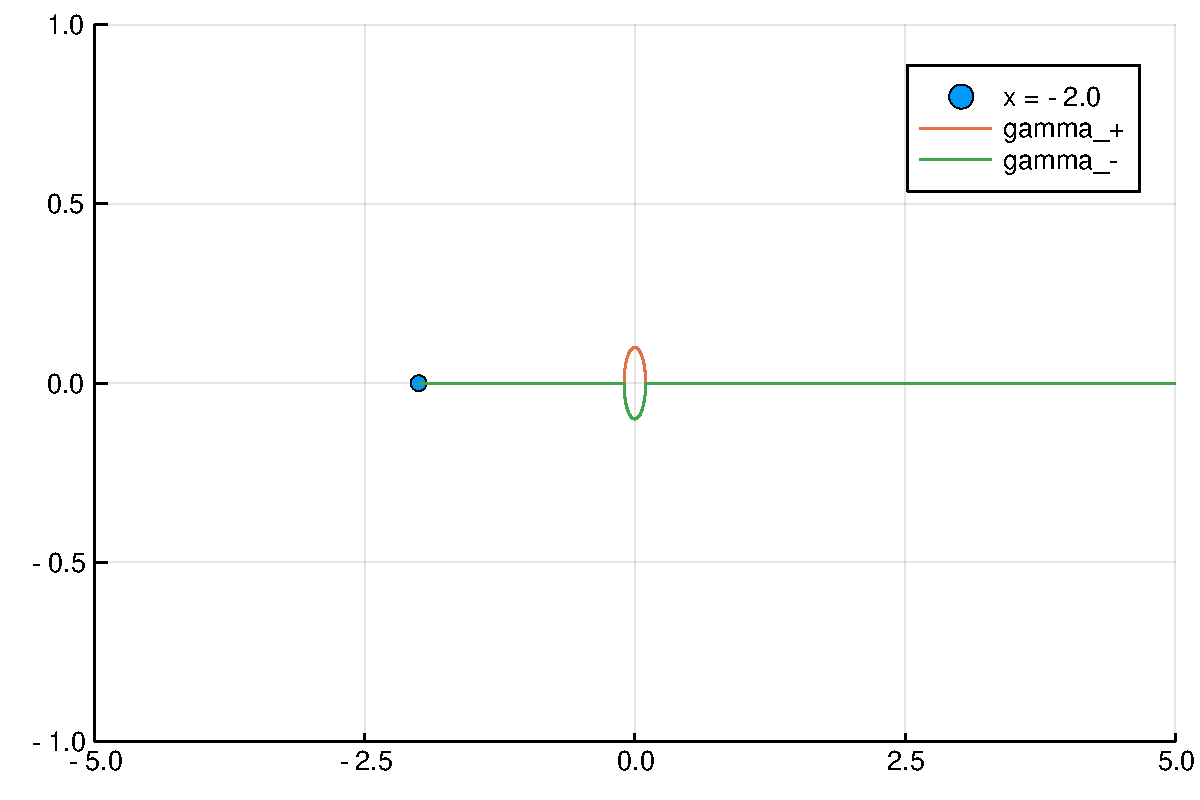
\includegraphics[width=\linewidth]{figures/Solutions3_7_1.pdf}

So that

\[
\Gamma_\pm(\alpha, x) = \int_{\gamma_{\pm x}} \zeta^{\alpha-1} \E^{-\zeta} \D \zeta
\]
Note that

\[
\int_x^{-r} (\zeta_+^{\alpha - 1} - \zeta_-^{\alpha -1}) \E^{-\zeta} \D\zeta = 0
\]
since $\zeta_+^{\alpha-1} = \E^{\pi \I (\alpha-1)}|\zeta|^{\alpha-1} = \E^{2 \I \pi \alpha} \zeta_-^{\alpha-1}$. Furthermore, the integrals over the arcs tend to zero as $r \rightarrow 0$:

\[
|\I r^\alpha \int_0^\pi \E^{- r \E^{\I \theta}} \E^{\I \theta \alpha} \D \theta  | \leq r^\alpha \pi \E^r  \rightarrow 0
\]
and similarly on the lower arc. Thus we have


\begin{align*}
\Gamma_+(\alpha, x)-\E^{2 \I \pi \alpha} \Gamma_-(\alpha, x) &= \lim_{r \rightarrow 0 } \left(\int_{\gamma_{+x}} - \E^{2 \I \pi \alpha} \int_{\gamma_{-x}}\right) \zeta^{\alpha-1} \E^{-\zeta} \D \zeta \ccr
 = (1 - \E^{2 \I \pi \alpha})\int_0^\infty x^{\alpha-1} \E^{-x} \dx = (1 - \E^{2 \I \pi \alpha})\Gamma(\alpha)
\end{align*}
\subsection{Problem 4.2}
Note that, for $0 < \alpha < 1$,

\[
    \psi(z) = z^{-\alpha} \E^z \Gamma(\alpha, z)
\]
has the following properties:

\begin{itemize}
\item[1. ] \[
\psi(z)
\]
decays as $z \rightarrow \infty$, via integration by parts:

\end{itemize}
\[
    z^{-\alpha} \E^z \int_z^\infty \zeta^{\alpha-1} \E^{-\zeta} \D \zeta =
    z^{-1} \E^z + z^{-\alpha} \int_z^\infty \zeta^{\alpha-2} \E^{z-\zeta} \D \zeta
\]
and we have assuming $z$ is bounded away from the negative real axis:

\[
\int_z^\infty \zeta^{\alpha-2} \E^{z-\zeta} \D \zeta| \leq \int_z^\infty |\zeta|^{\alpha-2} \D \zeta = \int_0^\infty |x+z|^{\alpha-2} \D x  < \infty
\]
(otherwise one would use a deformed contour). 

\begin{itemize}
\item[2. ] We have the subtractive jump:

\end{itemize}

\begin{align*}
\psi_+(x) - \psi_-(x) &= \E^x(x_+^{-\alpha} \Gamma_+(\alpha, x) -  \Gamma_-(\alpha, x)) \ccr
= \E^x |x|^\alpha (\E^{-\I \pi \alpha} \Gamma_+(\alpha, z) - \E^{\I \pi \alpha} \Gamma_-(\alpha,x)) \ccr
 = \E^x |x|^\alpha \E^{-\I \pi \alpha} (1-\E^{2 \I \pi \alpha})
\end{align*}
We use these properties to verify that

\[
\CC[\diamond^\alpha \E^{-\diamond}](z) = {1 \over \Gamma(-\alpha)} {(-z)^\alpha \E^{-z} \Gamma(-\alpha, - z) \over
  \E^{-\I\pi\alpha} - \E^{\I\pi\alpha}}
\]
via Plemelj.


\begin{lstlisting}
(*@\HLJLn{x}@*) (*@\HLJLoB{=}@*) (*@\HLJLnf{Fun}@*)(*@\HLJLp{(}@*)(*@\HLJLni{0}@*) (*@\HLJLoB{..}@*) (*@\HLJLnfB{20.0}@*)(*@\HLJLp{)}@*)
(*@\HLJLn{\ensuremath{\alpha}}@*) (*@\HLJLoB{=}@*) (*@\HLJLoB{-}@*)(*@\HLJLnfB{0.1}@*)
(*@\HLJLn{z}@*) (*@\HLJLoB{=}@*) (*@\HLJLnfB{2.0}@*)(*@\HLJLoB{+}@*)(*@\HLJLn{im}@*)
(*@\HLJLnf{cauchy}@*)(*@\HLJLp{(}@*)(*@\HLJLn{x}@*)(*@\HLJLoB{{\textasciicircum}}@*)(*@\HLJLn{\ensuremath{\alpha}}@*)(*@\HLJLoB{*}@*)(*@\HLJLnf{exp}@*)(*@\HLJLp{(}@*)(*@\HLJLoB{-}@*)(*@\HLJLn{x}@*)(*@\HLJLp{),}@*) (*@\HLJLn{z}@*)(*@\HLJLp{)}@*)

(*@\HLJLn{\ensuremath{\Gamma}}@*) (*@\HLJLoB{=}@*) (*@\HLJLp{(}@*)(*@\HLJLn{\ensuremath{\alpha}}@*)(*@\HLJLp{,}@*)(*@\HLJLn{z}@*)(*@\HLJLp{)}@*) (*@\HLJLoB{->}@*) (*@\HLJLk{let}@*) (*@\HLJLn{\ensuremath{\zeta}}@*) (*@\HLJLoB{=}@*) (*@\HLJLn{z}@*) (*@\HLJLoB{+}@*) (*@\HLJLnf{Fun}@*)(*@\HLJLp{(}@*)(*@\HLJLni{0}@*) (*@\HLJLoB{..}@*) (*@\HLJLnfB{500.0}@*)(*@\HLJLp{)}@*)
    (*@\HLJLnf{linesum}@*)(*@\HLJLp{(}@*)(*@\HLJLn{\ensuremath{\zeta}}@*)(*@\HLJLoB{{\textasciicircum}}@*)(*@\HLJLp{(}@*)(*@\HLJLn{\ensuremath{\alpha}}@*)(*@\HLJLoB{-}@*)(*@\HLJLni{1}@*)(*@\HLJLp{)}@*)(*@\HLJLoB{*}@*)(*@\HLJLnf{exp}@*)(*@\HLJLp{(}@*)(*@\HLJLoB{-}@*)(*@\HLJLn{\ensuremath{\zeta}}@*)(*@\HLJLp{))}@*)
(*@\HLJLk{end}@*)

(*@\HLJLoB{-}@*)(*@\HLJLp{(}@*)(*@\HLJLoB{-}@*)(*@\HLJLn{z}@*)(*@\HLJLp{)}@*)(*@\HLJLoB{{\textasciicircum}}@*)(*@\HLJLn{\ensuremath{\alpha}}@*)(*@\HLJLoB{*}@*)(*@\HLJLnf{exp}@*)(*@\HLJLp{(}@*)(*@\HLJLoB{-}@*)(*@\HLJLn{z}@*)(*@\HLJLp{)}@*)(*@\HLJLnf{\ensuremath{\Gamma}}@*)(*@\HLJLp{(}@*)(*@\HLJLoB{-}@*)(*@\HLJLn{\ensuremath{\alpha}}@*)(*@\HLJLp{,}@*)(*@\HLJLoB{-}@*)(*@\HLJLn{z}@*)(*@\HLJLp{)}@*)(*@\HLJLoB{/}@*)(*@\HLJLp{(}@*)(*@\HLJLnf{gamma}@*)(*@\HLJLp{(}@*)(*@\HLJLoB{-}@*)(*@\HLJLn{\ensuremath{\alpha}}@*)(*@\HLJLp{)}@*)(*@\HLJLoB{*}@*)(*@\HLJLp{(}@*)(*@\HLJLnf{exp}@*)(*@\HLJLp{(}@*)(*@\HLJLn{im}@*)(*@\HLJLoB{*}@*)(*@\HLJLn{\ensuremath{\pi}}@*)(*@\HLJLoB{*}@*)(*@\HLJLn{\ensuremath{\alpha}}@*)(*@\HLJLp{)}@*)(*@\HLJLoB{-}@*)(*@\HLJLnf{exp}@*)(*@\HLJLp{(}@*)(*@\HLJLoB{-}@*)(*@\HLJLn{im}@*)(*@\HLJLoB{*}@*)(*@\HLJLn{\ensuremath{\pi}}@*)(*@\HLJLoB{*}@*)(*@\HLJLn{\ensuremath{\alpha}}@*)(*@\HLJLp{)))}@*)
\end{lstlisting}

\begin{lstlisting}
0.07199876331505142 + 0.05850612396048861im
\end{lstlisting}



\end{document}
